%% Author - Matthew A Robson
\documentclass{beamer}
\usepackage{tikz}
\usepackage{quantikz}
\usepackage{textcomp}
\usepackage{amsmath}
\usepackage{hyperref}
\usepackage{physics}
\usepackage{graphicx}
\usetikzlibrary{positioning, angles, quotes}

\usetheme{Berkeley}
\usecolortheme{default}

%% I want to fix a few color and theme things to match my school
\definecolor{MySchoolBlue}{RGB}{0, 51, 102}
\setbeamercolor{structure}{fg=MySchoolBlue, bg=MySchoolBlue}
\setbeamercolor{item}{fg=MySchoolBlue}
\setbeamercolor{enumerate item}{fg=MySchoolBlue}
\setbeamercolor{itemize item}{fg=MySchoolBlue}


\title[Quantum Computing] %% includes the title on every slides
{High Speed Computing with Clustered and Quantum Computers}
\subtitle{}
\author[Robson, Matthew] %% includes my name on every slide
{M.~A.~Robson\inst{1}}

\institute[VFU] %% include the institution and further specifying information
{
  %\inst{1}%
  LASA{CS} Department\\
  Liberal Arts and Science Academy
  \and
  %\inst{2}%
  Period 1\\
  Independent Study Computer Science
}

\date[VLC 2021] %% include the date and even of the presentation
{Fall Final, December 2025}

\logo{
\begin{tikzpicture}
  \node (myImage) at (0,0) {\includegraphics[width=0.15\textwidth]{logo.png}};
\end{tikzpicture}
}

%End of title page configuration block
%------------------------------------------------------------
%The next block of commands puts the table of contents at the 
%beginning of each section and highlights the current section:

\AtBeginSection[]
{
  \begin{frame}
    \frametitle{Table of Contents}
    \tableofcontents[currentsection]
  \end{frame}
}
%------------------------------------------------------------
\begin{document}


%%%% Page 1 -- Title Page
\frame{\titlepage}

%%%% Page 2 -- Introduction 
\begin{frame}
\frametitle{What Is Quantum Computing?}

Quantum computing covers many concepts, but it is important to first start with classical computing.

\begin{block}{Classical Information}
In a classical computer it stores information as a 1 or a 0 in what is called a bit.
\end{block}

\begin{exampleblock}{Some Common Gates}
NAND, NOR, AND, OR, XOR $\rightarrow$ Complex structures such as ALUs and data storage.  
\end{exampleblock}

\begin{quantikz}
  \lstick{A} & \gate{NOT} & \rstick{$\bar{A}$}
\end{quantikz}

\end{frame}

%%%% Page 3 -- Time Complexity and Circuit Complexity
\begin{frame}
\frametitle{Circuit Complexity}

In circuits it is important to cover the complexity required to achieve certain goals.
Complexity is classified in Big O Notation.
\newline
\newline
Additionally, we can classify these further into P, NP, NP-complete, etc.

\begin{exampleblock}{Time Complexity Example}
  A loop of N elements has a time complexity of $\mathcal{O}(N)$.
\end{exampleblock}

\begin{alertblock}{Theorem 1.0}
  Any NP complete problem can be solve in polynomial time on a classical computer.
\end{alertblock}

\end{frame}

%%%% Page 4 -- Final Classical Computing 

\begin{frame}
\frametitle{Turing Completeness}

Simply, a Turing-complete computer is one that is able to compute any and Turing-computable function.

\begin{block}{Definition 1.0}
  Some computational device is taken as Turing-complete or Turing-equivalent if it is probable that it can compute the values for a function for every function of its argument.\ ie. A common place computer.
\end{block}

While Turing-complete computers are powerful, they begin to break down at the meta level in cases such as the infamous Halting Problem.\ (see the LASACS lunch time lecture)

\end{frame}

%%%% Page 5 -- Introduction to Quantum Computers and Qubits

\begin{frame}
\frametitle{A Single Qubit}

A single qubit is given by $\ket{\psi} = \alpha\ket{0} + \beta\ket{1}$.
\newline
\newline
$\alpha$ is given to be a number in the reals and $\beta$ is given to be a number in the complex space. Because of this we use a global phase to ensure $\alpha$ stays real.
\newline
\newline
\begin{block}{Definition 2.0}
  A qubit is best described by $\ket{\psi} = e^{i\gamma}(\alpha\ket{0} + \beta\ket{1}) | \alpha \epsilon 
  \mathbb{R}, \beta \epsilon \mathbb{C}$
\end{block}

\end{frame}



%%%% Page 6 -- Further Background on Qubits
\begin{frame}
\frametitle{Quantum Representation}

\begin{center}
  $\ket{\psi} = e^{i\gamma}(\alpha\ket{0} + \beta\ket{1}) | \alpha \epsilon \mathbb{R}, \beta \epsilon \mathbb{C}$
\end{center}

\centering %% Include the bloch sphere that I created for my notes
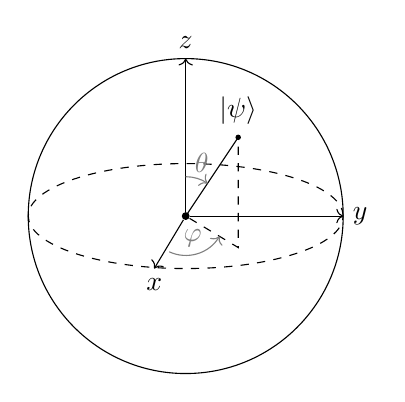
\begin{tikzpicture}

  % Define radius
  \def\r{2}

  % Bloch vector
  \draw (0,0) node[circle, fill, inner sep=1] (orig) {} -- (\r/3,\r/2)
    node[circle, fill, inner sep=0.7, label=above:$\ket{\psi}$] (a) {};
  \draw[dashed] (orig) -- (\r/3, -\r/5) node (phi) {} -- (a);

  % Sphere
  \draw (orig) circle (\r);
  \draw[dashed] (orig) ellipse (\r{} and \r/3);

  % Axes
  \draw[->] (orig) -- ++(-\r/5, -\r/3) node[below] (x1) {$x$};
  \draw[->] (orig) -- ++(\r, 0) node[right] (x2) {$y$};
  \draw[->] (orig) -- ++(0, \r) node[above] (x3) {$z$};

  % Angles
  \pic [draw=gray, text=gray, ->, "$\varphi$"] {angle = x1--orig--phi};
  \pic [draw=gray, text=gray, <-, "$\theta$", angle eccentricity=1.4] {angle = a--orig--x3};

\end{tikzpicture}

$\alpha = \cos{\frac{\theta}{2}}$\\
$\beta  = e^{i\varphi}\sin{\frac{\theta}{2}}$

\end{frame}


%%%% Page 7 -- Linear Algebra Crash Course

\begin{frame}
\frametitle{Linear Algebra Crash Course}

In terms of our qubit we can define some vectors to represent our previous kets for 0 and 1:
\[
    \ket{0}=
    \begin{pmatrix}
    1 \\
    0
    \end{pmatrix}
    ,
    \ket{1}=
    \begin{pmatrix}
    0 \\
    1
    \end{pmatrix}
\]
Plugging this into our previous formulas we can see: 
\[
    \ket{\psi} = \alpha\begin{pmatrix} 1 \\ 0 \end{pmatrix} + \beta\begin{pmatrix} 0 \\ 1 \end{pmatrix} = \begin{pmatrix} \alpha \\ \beta \end{pmatrix}
\]
We rewrite all of this work we have done in terms of vectors because it allows for our later use of matrices to act as the gates and for massively parallelized work.

\end{frame}



%%%% Page 8 -- Linear Algebra cont.
\begin{frame}
\frametitle{More Linear Algebra}

Now with the use of these vectors we can perform some algebraic operations such as the tensor product allowing for us to combine gates and qubits.
\[
    \begin{pmatrix}
        \alpha & \beta\\
        \gamma & \delta
    \end{pmatrix}
    \otimes
    \begin{pmatrix}
        A & B\\
        \Gamma & \Delta
    \end{pmatrix}
    =
    \begin{pmatrix}
        \alpha 
        \begin{pmatrix}
            A & B\\
            \Gamma & \Delta
        \end{pmatrix} 
        & \beta
        \begin{pmatrix}
            A & B\\
            \Gamma & \Delta
        \end{pmatrix}
        \\
        \gamma
            \begin{pmatrix}
            A & B\\
            \Gamma & \Delta
        \end{pmatrix}
        & \delta
        \begin{pmatrix}
            A & B\\
            \Gamma & \Delta
        \end{pmatrix}
    \end{pmatrix}
    =
\]
\[
    \begin{pmatrix}
        \alpha A      & \alpha B      & \beta A      & \beta   B      \\
        \alpha \Gamma & \alpha \Delta & \beta \Gamma & \beta   \Delta \\
        \gamma A      & \gamma B      & \delta A     & \delta  B      \\
        \gamma \Gamma & \gamma \Delta & \delta \Gamma & \delta \Delta         
    \end{pmatrix}
\]

\end{frame}



%%%% Page 9 -- Basic Quantum Gates
\begin{frame}
\frametitle{Quantum Gates}

\begin{block}{What are Quantum Gates?}
  A quantum gate like a classical gate changes the state of a piece of information. Unlike many classical gates, a quantum gate is always reversible.
\end{block}


\begin{exampleblock}{Pauli-X Gate}
\begin{center}
  \begin{quantikz}
    \lstick{$\ket{0}$} & \gate{X} & \rstick{$\ket{1}$}
  \end{quantikz}
\end{center}
The Pauli-X gate acts in a similar fashion to that of a classical not gate.
\end{exampleblock}


\end{frame}


%%%% Page 10 -- Quantum Axis
\begin{frame}
\frametitle{Quantum Measurement}

\centering
\begin{tikzpicture}

  % Define radius
  \def\r{3}


  % Sphere
  \draw (orig) circle (\r);
  \draw[dashed] (orig) ellipse (\r{} and \r/3);

  % X-axis (Red)
  \draw[->, red] (orig) -- ++(-\r/5, -\r/3) node[below] {$\ket{+}$};
  \draw[->, red] (orig) -- ++(\r/5, \r/3) node[above] {$\ket{-}$};

  % Y-axis (Green)
  \draw[->, green!60!black] (orig) -- ++(\r, 0) node[right] {$\ket{+i}$};
  \draw[->, green!60!black] (orig) -- ++(-\r, 0) node[left] {$\ket{-i}$};

  % Z-axis (Blue)
  \draw[->, blue] (orig) -- ++(0, \r) node[above] {$\ket{0}$};
  \draw[->, blue] (orig) -- ++(0, -\r) node[below] {$\ket{1}$};

\end{tikzpicture}
\end{frame}


%%%% Page 11 -- Quantum Axis Conversion
\begin{frame}
% \begin{tikzpicture}

%   % Define radius
%   \def\r{1}


%   % Sphere
%   \draw (orig) circle (\r);
%   \draw[dashed] (orig) ellipse (\r{} and \r/3);

%   % X-axis (Red)
%   \draw[->, red] (orig) -- ++(-\r/5, -\r/3) node[below] {$\ket{+}$};
%   \draw[->, red] (orig) -- ++(\r/5, \r/3) node[above] {$\ket{-}$};

%   % Y-axis (Green)
%   \draw[->, green!60!black] (orig) -- ++(\r, 0) node[right] {$\ket{+i}$};
%   \draw[->, green!60!black] (orig) -- ++(-\r, 0) node[left] {$\ket{-i}$};

%   % Z-axis (Blue)
%   \draw[->, blue] (orig) -- ++(0, \r) node[above] {$\ket{0}$};
%   \draw[->, blue] (orig) -- ++(0, -\r) node[below] {$\ket{1}$};

% \end{tikzpicture}

It can be seen that the $\ket{+i}, \ket{-i}, \ket{-}, \ket{+}$ all fall along the equator of the bloch sphere. We can represent these points on the sphere using the following formulas:
\begin{exampleblock}{Basis}
  $\ket{+} = \frac{1}{\sqrt{2}}(\ket{0} + \ket{1})$\\
  $\ket{-} = \frac{1}{\sqrt{2}}(\ket{0} - \ket{1})$\\
  $\ket{+i} = \frac{1}{\sqrt{2}}(\ket{0} +i \ket{1})$\\
  $\ket{-i} = \frac{1}{\sqrt{2}}(\ket{0} -i \ket{1})$
\end{exampleblock}
It is trivial to see how this concept can be extended to further to any arbirary basis. 


\end{frame}


\begin{frame}

\end{frame}


\end{document}
